% Figures for the revised paper, generated from results/data/runs_v2.csv by
% scripts/plotting/paper_figures.py. Compile standalone:
%     cd paper && pdflatex figures.tex
% To drop into the paper: copy each figure environment (and the \usepackage{float}
% line) into the manuscript; \graphicspath points at paper/figures/.
\documentclass[10pt]{article}
\usepackage[letterpaper,textwidth=5.5in,textheight=9in]{geometry}
\usepackage{graphicx}
\usepackage{float}
\usepackage{xcolor}
\usepackage{amsmath,amssymb}
\usepackage[font=small,labelfont=bf,skip=4pt]{caption}
\usepackage{times}
\usepackage{booktabs}
\graphicspath{{figures/}}
\newcommand{\replaces}[1]{\vspace{-4pt}\noindent{\footnotesize\color{gray}#1}\par\bigskip}
\newcommand{\tfc}{t_{\mathrm{first\,cross}}}
\newcommand{\tmemo}{t_{\mathrm{memo}}}
\setlength{\parindent}{0pt}
\setlength{\parskip}{4pt}

\begin{document}

{\Large\bfseries Federated learning and grokking: revised figures}\\[2pt]
{\small Regenerated from the v2 corpus (1{,}685 runs, five setups). Every number in a caption is computed by the plotting script and written to \texttt{figures/figure\_numbers.json}. Figures are sized to the 5.5\,in text width; each is pinned with \texttt{[H]} so it stays next to the text that describes it. Throughout, points are Kaplan--Meier medians over runs, error bars span the minimum to maximum over runs, a hollow marker means not every run held the bar to the end, and a cross means no run reached the event within budget (``failed to grok'').}

\medskip
\begin{tabular}{@{}p{1.0in}p{0.65in}p{3.4in}@{}}
\toprule
Draft figure (1 Sep) & Replaced by & Change \\
\midrule
Fig.\ 1 slowdown vs $K$ & Fig.\ 1 & panel (a) re-drawn on v2; the $K{=}97$ point is now 2/5 at the budget, not $>2\times$; (b, c) add the two clocks \\
Fig.\ 2 heterogeneity & Fig.\ 4 & anchor is flat (a); the 0.01 delay was starvation (c); thresholds are per architecture (b) \\
Fig.\ 3 local epochs & Fig.\ 2 & anchor curve reproduced (a); transformers pay in memorisation, flat in rounds (b) \\
Fig.\ 4 participation & Fig.\ 3 & null reproduced in rounds; divergence panel added; MNIST exception \\
Fig.\ 5 drift & Fig.\ 5(a) & same scatter; three zero-cost axes and two interventions separate signature from cause \\
Fig.\ 6 norm ratio, IPR & Fig.\ 7 & IPR kept with temporal order; layer-norm ratio dropped (v1 only) \\
Fig.\ 7 $T_{\mathrm{grok}}$ vs $T_{\mathrm{mem}}$ & Fig.\ 1 & the decomposition is the spine \\
Fig.\ 8 optimisers & Fig.\ 5(b--d) & every method at its calibrated server LR; the weight-decay column deleted (values bug) \\
Fig.\ 9 fingerprints & Fig.\ A2 & first-crossing time per method and cell \\
--- & Fig.\ 6 & new: the fixed point \\
\bottomrule
\end{tabular}

\bigskip

% ── Fig 1 ────────────────────────────────────────────────────────────────────
\begin{figure}[H]
  \centering
  
\includegraphics[width=\textwidth]{fig1_two_clocks.pdf}
  \caption{\textbf{Federation costs memorisation time plus a delay, and the optimiser decides which term pays.}
  (a)~Ratio of federated to centralised first-crossing time on setup A (quadratic MLP, $a{+}b \bmod 97$, GD) against the number of clients $K$ under IID sharding, at two training fractions; error bars span the runs, marker fill is the fraction of runs whose bar held to the end. Fifty clients cost 17\% at $\alpha{=}0.30$. At $\alpha{=}0.25$, $K{=}97$ crosses in 2 of 5 runs, both within 5\% of the 100k-step budget, while the operand split (square) crosses in 5 of 5 at 76{,}100 steps.
  (b,~c)~Kaplan--Meier median time to memorise (train accuracy $\ge 99\%$) and median memorise-to-generalise delay against $K$ on A (GD, no decay), B (transformer on $a{+}b \bmod 113$, AdamW, wd~0.1) and D (quadratic MLP on $S_5$, AdamW, wd~1.0), all at $\alpha{=}0.30$. Under GD memorisation is flat and the delay grows; under AdamW the delay is roughly constant and memorisation itself explodes with $K$ (B: 150 $\to$ 3{,}600 $\to$ 53{,}300 steps at $K{=}1, 20, 50$). A cross on the top edge marks a cell where no run reached the event within budget. All five setups and B's inherited decay are in Fig.~\ref{fig:A1}.}
  \label{fig:two-clocks}
\end{figure}
\replaces{Replaces draft Fig.~1. Withdraw ``in the most extreme setting the slowdown exceeds $2\times$''; the $K{=}97$ point was read off a 50k budget on a cell that needs $\sim$97k.}

% ── Fig 2 ────────────────────────────────────────────────────────────────────
\begin{figure}[H]
  \centering
  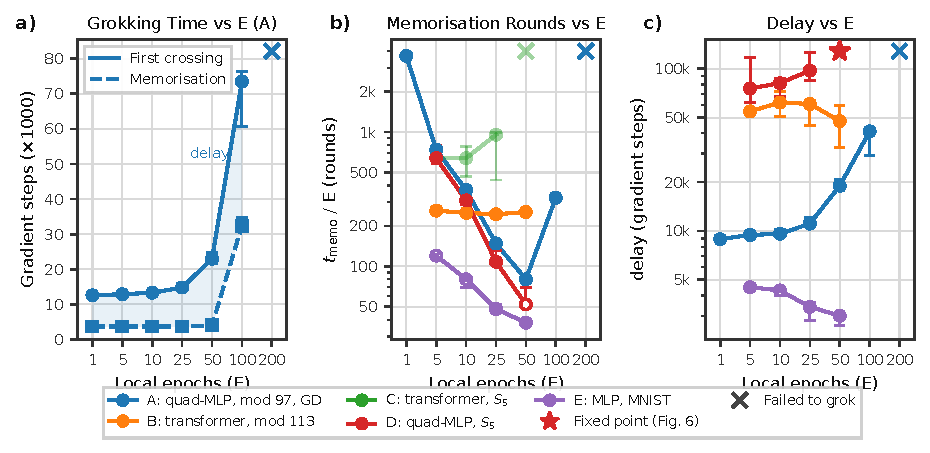
\includegraphics[width=\textwidth]{fig2_local_work.pdf}
  \caption{\textbf{Local work taxes a different phase on each architecture.} Compute-matched: rounds scale as $5/E$ so every rung does the same gradient work; $K{=}10$, IID.
  (a)~Setup A: time to memorise (dashed) and time to first crossing (solid) against local epochs $E$; the shaded gap is the delay, which grows $2.1\times$ from $E{=}1$ to 50 while memorisation is flat. The $E{=}1$ rung reproduces the centralised run to the step (FedAvg at $E{=}1$ is an identity with centralised GD).
  (b)~Time to memorise in aggregation rounds ($\tmemo/E$): flat on the transformers B and C ($\approx$250 rounds at every $E$ on B), so it scales linearly with $E$ in steps; falls as $1/E$ on the quadratic MLPs A and D, so it is flat in steps. Weight decay is not the reason: D carries ten times B's decay and does not move.
  (c)~Delay in steps: grows on A, does not move on B, grows on D until $E{=}50$ enters the fixed point of Fig.~\ref{fig:fixed-point} (star). C's delay is $\approx 0$ from $E{=}25$ and its numbers are withheld (Limitations).}
  \label{fig:local-work}
\end{figure}
\replaces{Replaces draft Fig.~3. Withdraw ``in low-data boundary regimes, large $E$ can prevent grokking entirely within the training budget'': those cells were censored on A and are the fixed point on D.}

% ── Fig 3 ────────────────────────────────────────────────────────────────────
\begin{figure}[H]
  \centering
  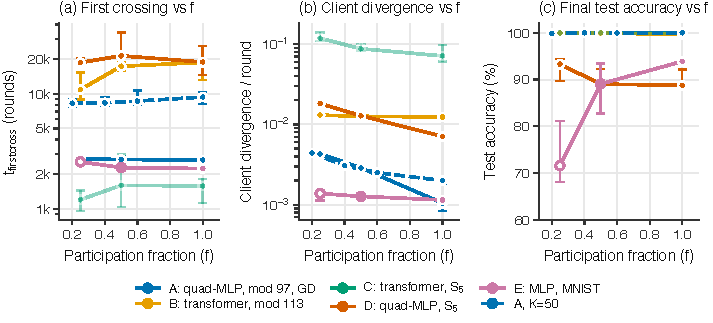
\includegraphics[width=\textwidth]{fig3_participation.pdf}
  \caption{\textbf{Partial participation is free per communication round.} $K{=}20$, IID, $E{=}5$; rounds scale as $1/f$ so every cell does the same gradient work as its $f{=}1$ control (dashed: A at $K{=}50$). Read in rounds: the step axis halves with $f$ by construction.
  (a)~First crossing in rounds is flat in $f$ on every setup; A's delay is 1{,}920 rounds at every $f$. B's delay shortens $1.8\times$ at $f{=}0.25$ (one setup, $2$--$3\times$ run spread).
  (b)~Client weight divergence per round, averaged before the first crossing, rises as $f$ falls ($1.8\times$ on A) at no cost in rounds; this is the intervention Fig.~\ref{fig:drift} needs, because $f$ moves disagreement without touching $K$, $E$ or the data.
  (c)~Final test accuracy moves only on MNIST, $94 \to 72\%$, measured at its degenerate $K{=}20$ (one full-batch step per local epoch); A, B and C end at 100\% and D at 89--93\% at every $f$.}
  \label{fig:participation}
\end{figure}
\replaces{Replaces draft Fig.~4. The null holds; the draft's step axis was inflated $\sim$2.5$\times$ by the old \texttt{total\_steps} accounting.}

% ── Fig 4 ────────────────────────────────────────────────────────────────────
\begin{figure}[H]
  \centering
  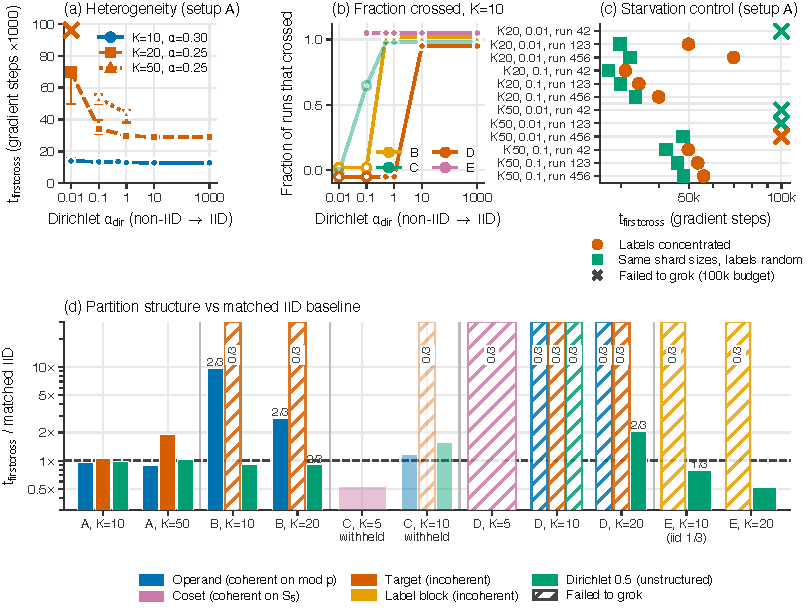
\includegraphics[width=\textwidth]{fig4_heterogeneity_structure.pdf}
  \caption{\textbf{Heterogeneity has a threshold per architecture; the anchor's apparent slowdown was client starvation; coherent structure helps on some setups and incoherent structure hurts everywhere.}
  (a)~Setup A, first-crossing time against Dirichlet concentration. At $K{=}10$, $\alpha{=}0.30$ (solid) the curve is flat across five orders of magnitude (18/18 runs, $1.09\times$). The $\alpha{=}0.25$ arms at $K{=}20$ and $50$ (dashed, dotted) slow or fail only at the rungs where the smallest shard holds $\le 2$ samples.
  (b)~Fraction of runs that crossed the bar at $K{=}10$ on B, C, D and E (lines offset vertically by a few hundredths so they can be told apart); hollow markers never memorised (peak train $< 99\%$). B and C fail by not memorising below $\alpha_{\mathrm{dir}} \approx 0.5$; D memorises fully at 0.5 and 1.0 and never generalises (the equilibrium of Fig.~\ref{fig:fixed-point}); E is unaffected.
  (c)~The starvation control on A at $\alpha{=}0.25$: the same shard sizes with labels randomised (squares) fail on exactly the runs whose smallest client holds $\le 2$ samples, so the failure is starvation, not label skew. The surviving label cost is $\sim$15\% at $\alpha_{\mathrm{dir}}{=}0.1$.
  (d)~First-crossing time of each structured partition divided by an exactly matched IID baseline (same setup, $K$, $\alpha$, width, budget); hatched bars to the top are cells where no run crossed. Coherent sharding beats random shards on A ($0.89\times$ at $K{=}50$) and on C, loses on B and D; the incoherent target split is the worst partition on every setup. C's bars are faded: its numbers are withheld.}
  \label{fig:heterogeneity}
\end{figure}
\replaces{Replaces draft Fig.~2 and the partition sentence in \S3.2.2. Withdraw ``under extreme heterogeneity grokking is noticeably delayed'' and ``the precise partition structure has little effect''.}

% ── Fig 5 ────────────────────────────────────────────────────────────────────
\begin{figure}[H]
  \centering
  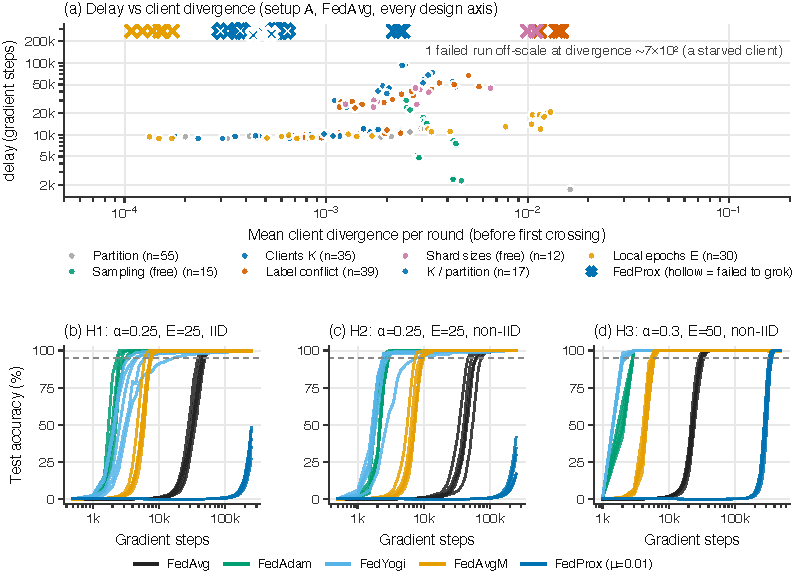
\includegraphics[width=\textwidth]{fig5_drift_mitigation.pdf}
  \caption{\textbf{Client drift is a signature, not the cause; adaptive server optimisers are 10--20$\times$ faster than FedAvg once every method is calibrated.}
  (a)~Memorise-to-generalise delay against mean client weight divergence per round, averaged over the window before the first crossing, for every FedAvg run on setup A, coloured by the design axis that produced it. Subsampling clients and unequal shard sizes raise divergence at no cost; label conflict raises it and costs time; SCAFFOLD (diamonds) sits at high pre-crossing divergence with a short delay; FedProx (crosses) at low divergence is censored. Reducing drift is therefore neither necessary nor sufficient.
  (b--d)~Test-accuracy trajectories on the three hard cells, five runs per method, each method at its own calibrated server learning rate (FedAdam and FedYogi 0.1, FedAvgM 1.0 with momentum 0.9). FedAdam and FedYogi cross at 2{,}000--5{,}000 steps against FedAvg's 31{,}000--61{,}000; SCAFFOLD is third and FedAvgM fourth; FedProx at $\mu{=}0.01$ is censored on H1 and H2 and $11\times$ slower than FedAvg on H3. Kaplan--Meier medians per method are in Fig.~\ref{fig:A2}. Server learning rates were calibrated at $E{=}5$ and applied at $E{=}25$ and $50$.}
  \label{fig:drift}
\end{figure}
\replaces{Replaces draft Figs.~5, 8 and 9. Withdraw ``client drift is the main federated perturbation''; delete the weight-decay column of Fig.~8 (it ran $\mathrm{lr}\cdot\lambda \in \{0.5, 5, 50\}$).}

% ── Fig 6 ────────────────────────────────────────────────────────────────────
\begin{figure}[H]
  \centering
  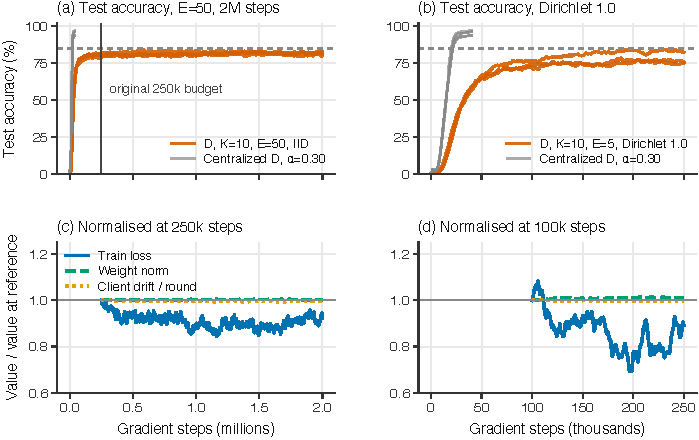
\includegraphics[width=0.95\textwidth]{fig6_fixed_point.pdf}
  \caption{\textbf{Setup D reaches a federated equilibrium that memorises perfectly and never generalises.}
  Left: $K{=}10$, $E{=}50$, IID, three runs to 2{,}000{,}000 steps, eight times the original budget (vertical line). Right: $K{=}10$, $E{=}5$, Dirichlet 1.0, three runs to 250{,}000 steps.
  (a,~b)~Test accuracy with the 85\% bar; centralised D (grey) groks at 21{,}300 steps.
  (c,~d)~Train loss, weight norm and client drift per round, each divided by its value at the reference step and shown as the median over runs from that step onward. Weight norm and drift are stationary within 1\% (left: 101.5 $\to$ 101.6 and 8.0 $\to$ 8.0 over 1.75M steps); train loss drifts down by $\sim$8\% on the left and is still falling slowly on the right, and never falls below 0.055, so the gradient is alive. Decay at wd~1.0 is alive; each round's local epochs drift the clients $\sim$8 units and averaging pulls them back, and the forces balance. The same state is reached from two axes that share nothing but the setup, which makes it a property of the setup rather than of one cell.}
  \label{fig:fixed-point}
\end{figure}
\replaces{New. The first breakdown in the study to survive a longer budget. Whether it belongs to $S_5$ or to AdamW on a quadratic MLP, and whether the per-round optimiser reset is load-bearing, are the open controls.}

% ── Fig 7 ────────────────────────────────────────────────────────────────────
\begin{figure}[H]
  \centering
  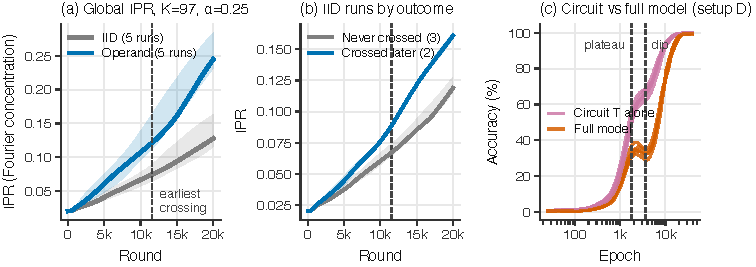
\includegraphics[width=\textwidth]{fig7_mechanism.pdf}
  \caption{\textbf{Coherent shards build Fourier structure before they generalise, and the same measure orders random-shard runs by their outcome.}
  (a)~Per-neuron spectral IPR of the global first layer, $K{=}97$, $\alpha{=}0.25$; median and range over five runs per arm. The operand arm separates completely from IID by round 6{,}000, 5{,}600 rounds before the earliest first crossing in the cell (vertical line). Under the operand split each first-operand column is trained by exactly one client, so a periodic pattern across columns requires the clients to agree: the global spectrum is a consensus measure there.
  (b)~Within the IID arm, the two runs that eventually cross separate from the three that never do from round 6{,}000 onward ($n{=}5$).
  (c)~Setup D at $\alpha{=}0.40$, centralised: accuracy of the compositional circuit $T$ alone against the full model's test accuracy. $T$ keeps improving through the mid-training dip while the full model falls, so the dip is masking by the marginal terms, not a loss of structure.}
  \label{fig:mechanism}
\end{figure}
\replaces{Replaces draft Figs.~6 and 7. IPR is kept, now with temporal order; the layer-norm ratio panels were v1 data on one setup and are dropped.}

\clearpage
{\large\bfseries Appendix figures}
\setcounter{figure}{0}
\renewcommand{\thefigure}{A\arabic{figure}}

\begin{figure}[H]
  \centering
  
\includegraphics[width=\textwidth]{figA1_two_clocks_all_setups.pdf}
  \caption{\textbf{The two clocks on every setup.} Kaplan--Meier median time to memorise (top) and median delay (bottom) against $K$, FedAvg, IID, $E{=}5$, at each setup's working point (solid) and its second series (dashed: another $\alpha$, or B's inherited wd~1.0). C is drawn faded and its numbers are withheld; E stops at $K{=}20$. Under B's inherited decay the delay collapses to $\sim$300 steps and the whole question is whether the model memorises at all; C's delay collapses with $K$ and at $K{=}50$ the first crossing precedes memorisation.}
  \label{fig:A1}
\end{figure}

\begin{figure}[H]
  \centering
  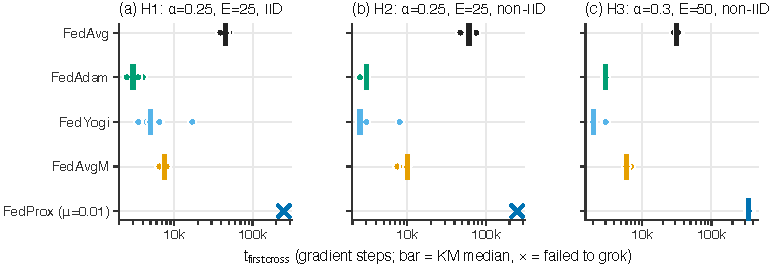
\includegraphics[width=\textwidth]{figA2_algorithms_first_crossing.pdf}
  \caption{\textbf{First-crossing time per method and cell.} Five runs per method; the bar is the Kaplan--Meier median, crosses are runs censored at the budget. H1: $\alpha{=}0.25$, $K{=}10$, $E{=}25$, IID. H2: same, Dirichlet 0.1. H3: $\alpha{=}0.30$, $K{=}10$, $E{=}50$, Dirichlet 0.1. The ordering is identical on $t_{\mathrm{grok}}$.}
  \label{fig:A2}
\end{figure}

\end{document}
